%%%%%%%%%%%%%%%%%%%%%%%%%%%%%%%%%%%%%%%%%%%%%%%%%
%%%%%%%%%%%% cap: installer %%%%%%%%%%%%%%%%%
%%%%%%%%%%%%%%%%%%%%%%%%%%%%%%%%%%%%%%%%%%%%%%%%%

\chapter{Creating an App Installer for the Platform}\label{cap:installer}
The platform solution proposed in this paper has strict requirements when it comes to the folder hierarchy employed by the platform itself. All applications are stored at a specific location; said location can be hard to find for the end-user that is not experienced with navigating the Windows file system. To combat this lack of ease of use in less experienced users, this solution also implements another tool, an installation wizard, to serve as a means to install applications automatically instead of manually doing so through the Windows File Explorer.


\section{Installer Architecture} \label{sect: Installer architecture}
The installer is a Microsoft Foundation Class (MFC) type application. MFC was used to create the user interface for the installer and to make it easily exportable and compatible with all Windows platforms. The installer has 2 functions. It can install the platform itself, at any location the user chooses, and it can install individual apps [see fig. \ref{fig:Installer Use Case Diagram}]. The interface dialog allows the user to select individual applications to be installed via Check-Box Control type items. It then installs all of the selected applications using \textit{.bat} scripts that come with the installer itself which issue download requests to GitHub.

\begin{figure}[H]
  \centering
  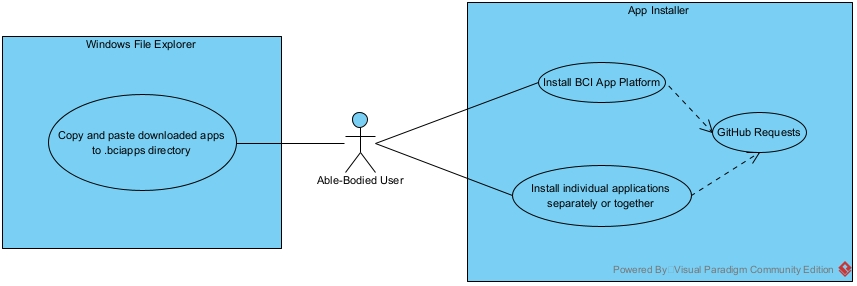
\includegraphics[width=1\textwidth]{Diagrams/Use Case/Installer.jpg}
  \caption{Installer Use Case Diagram}
  \label{fig:Installer Use Case Diagram}
\end{figure}


\section{Implementation Details} \label{sect: Installer implementation}
The installer is a dialog-based MFC app built using the Visual Studio IDE and its visual C++ tools. The dialog and all controller logic are written in C++, while external \textit{.bat} files are used via system calls to issue the download and file manipulation commands inside the file system.

\subsection{MFC Application} \label{subsect: Installer MFC application}
The MFC dialog consists of two parts, namely the platform installer and the application installer. Separated in their own group boxes, the parts each have their own controllers. The platform installation has an Edit Control to display the current installation path of the BCI App platform (which defaults to the user's Program Files directory each time the application starts) and two buttons, one labelled browse which serves as a way for the user to browse for his/her preferred directory and an install button, which calls the \textit{.bat} file that installs the platform. The second part, the app installer, consists of multiple check-boxes, each corresponding to its own application, from which one may pick the items they want and an install button that also uses a system call for the installation batch files. 

\subsection{Batch Files} \label{subsect: Installer batch files}
To download and install anything, a batch file is used to send a download request to GitHub via the curl command. All compatible apps and the platform respectively have their binary files on separate GitHub releases, which can be fetched with the aforementioned commands. Each download is stored in the user's temporary files directory, inside a .zip file. The file is then extracted to its respective output path, either the .bciapps folder for applications or the user's preferred directory for the platform, after which the temporary download file is deleted so as not to consume space on the local user's disk [see fig. \ref{fig:installer workflow}]. In the case of an error, the program is simply not installed and the user can check the logs to see at which step of the process the installation failed.

\begin{figure}[H]
  \centering
  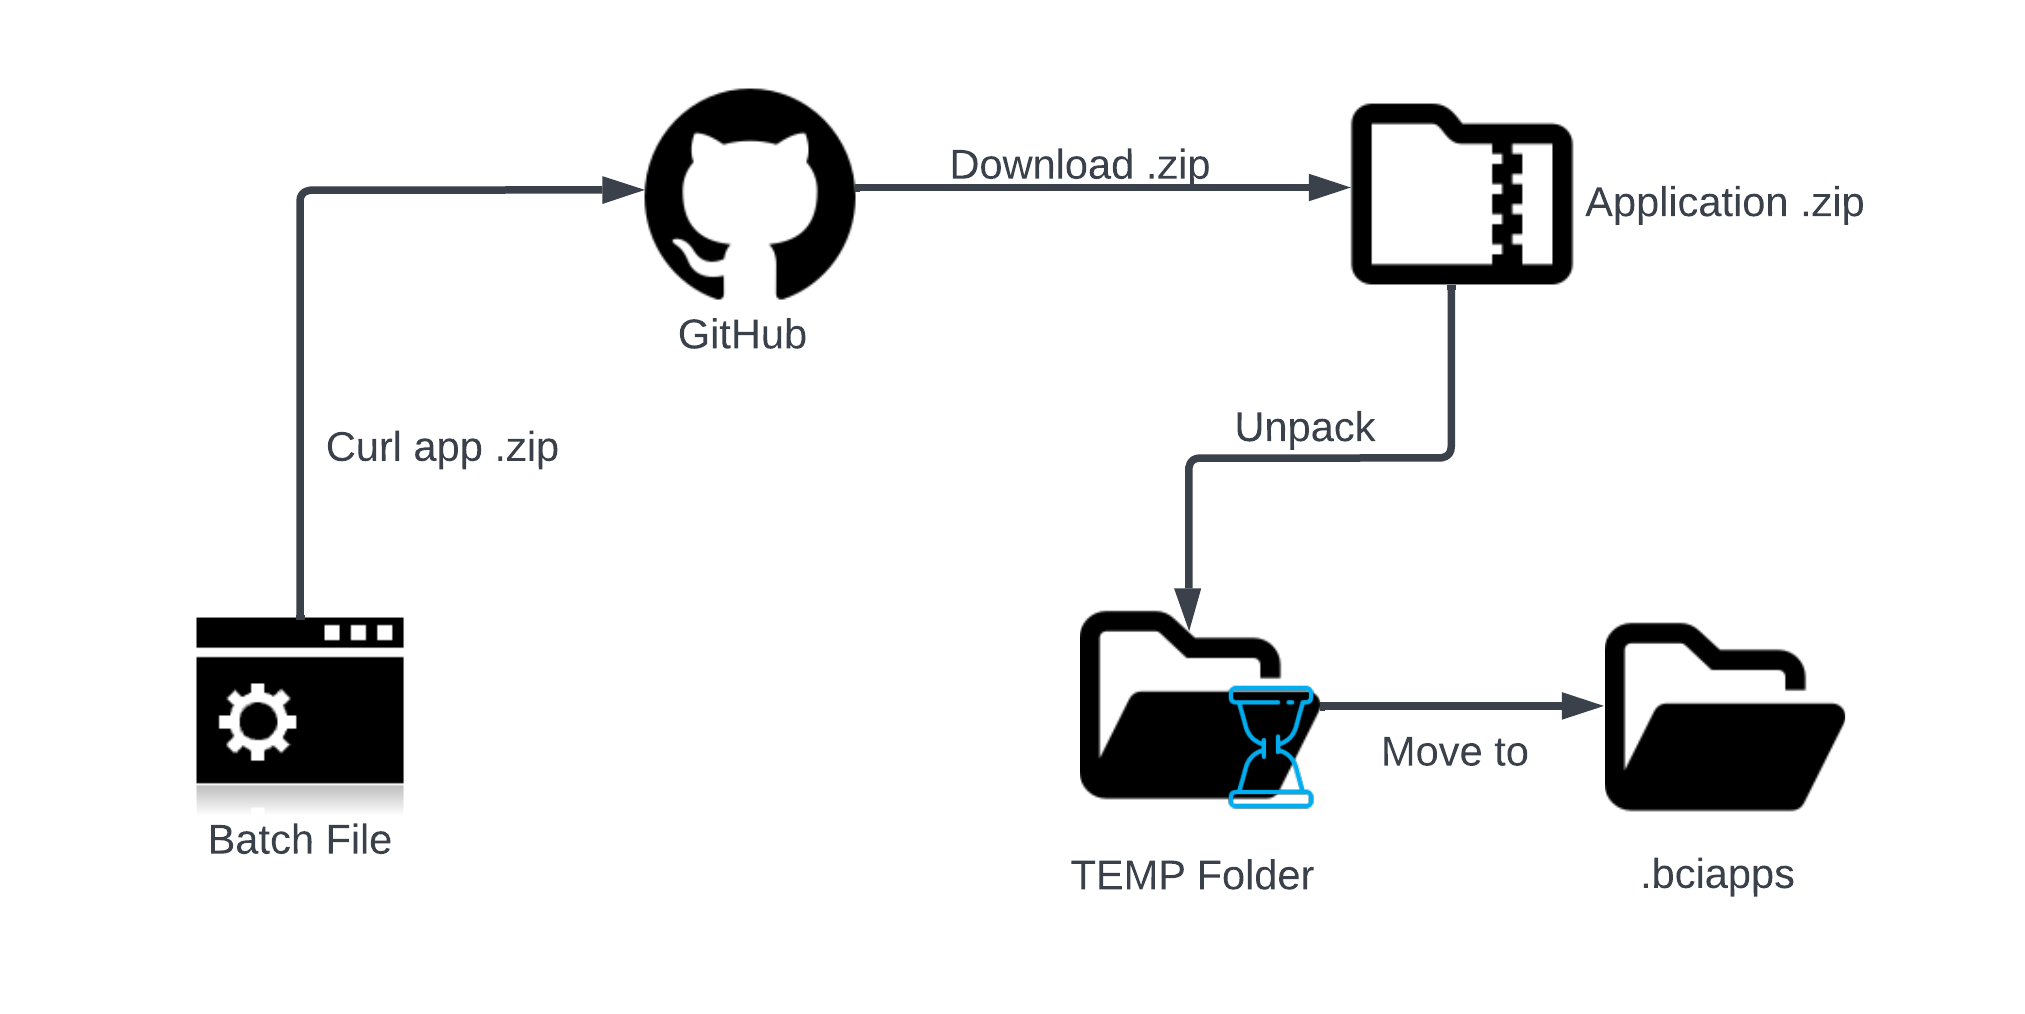
\includegraphics[width=1\textwidth]{Diagrams/Installer Workflow.png}
  \caption{Installer file workflow}
  \label{fig:installer workflow}
\end{figure}


When it comes to installing the applications the user selected via the checkboxes in the MFC dialog, a main installer.bat script is called alongside multiple arguments. Each argument represents a code for a specific program to be installed. The installer.bat script loops through all arguments and checks whether they correspond to a compatible app inside the GitHub releases. If it does, it executes the specific batch file for installing that application [see fig. \ref{fig:installer sequence diagram}].

\begin{figure}[H]
  \centering
  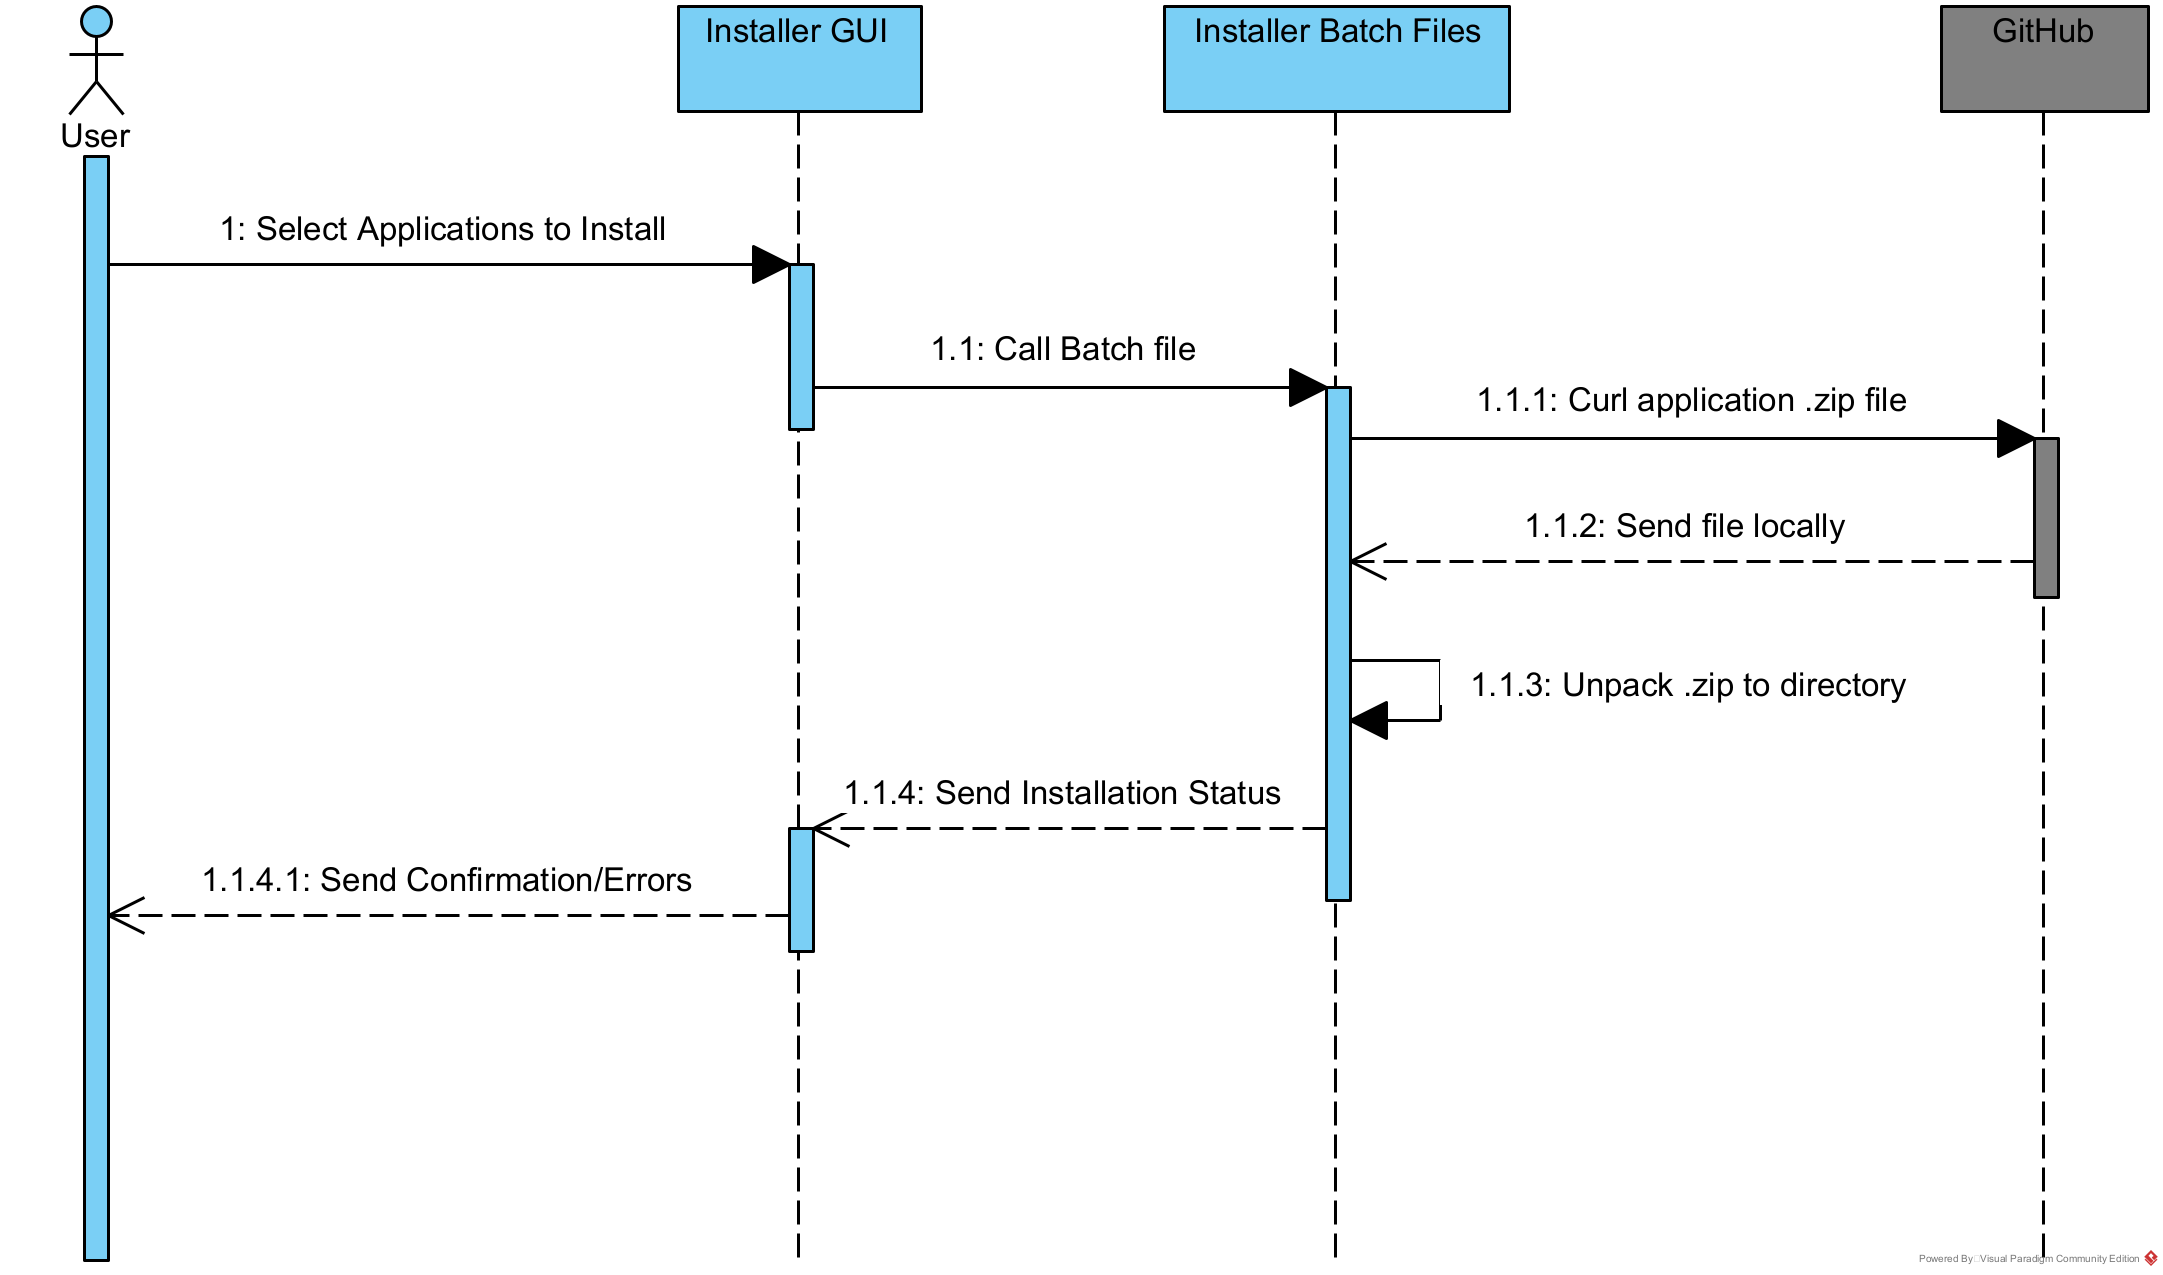
\includegraphics[width=1\textwidth]{Diagrams/Sequence/Installer.png}
  \caption{Installer sequence diagram}
  \label{fig:installer sequence diagram}
\end{figure}

\subsection{Updatability and Alternatives}
As with any installer, as new applications roll out, the installer will become outdated, at which point the user can simply head to the GitHub repository for the installer and grab the latest release, containing the new applications. Furthermore, the installer tool is easily modifiable when it comes time for an update. Whenever a new application rolls out, a new checkbox can be added inside the dialog, a new batch script is added for curling the download URL and the modification is made inside of the Action Handler for the install button. While it may be more intuitive to run the batch files on their own or just manually download the app releases, this tool is a solution for the less technologically savvy people who want to use the platform quickly and don't want to bother with the technicalities of separate downloads or unknown scripts but instead would opt for a more user-friendly experience.
\vspace{\baselineskip}\newline
An alternative to using the installer would be to install applications by hand, or to place one's applications inside the \textit{.bciapps} folder. This is useful for developers or people who use personal applications alongside the platform, but each application needs to respect the folder structure as presented in section \ref{sect:Platform Folder Structure}. As long as the structure is respected, any applications can be manually installed by an able-bodied user to be used alongside the Unicorn BCI.


\section{Graphical Interface} \label{sect:Installer GUI}
\begin{figure}[H]
    \begin{minipage}[c]{0.45\linewidth}
      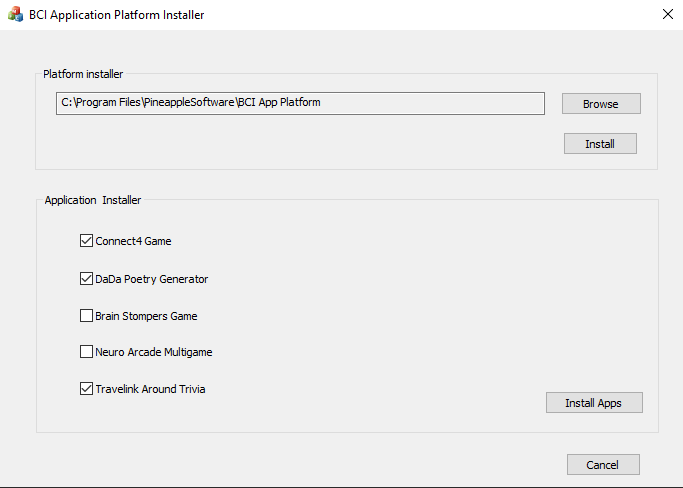
\includegraphics[width=\linewidth]{Graphics/Installer GUI.png}
      \caption{Installer Dialog Window}
      \end{minipage}
    \hfill
    \begin{minipage}[c]{0.45\linewidth}
      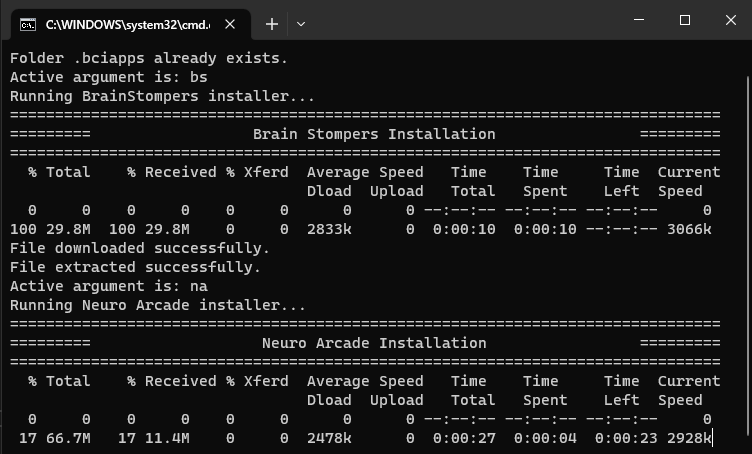
\includegraphics[width=\linewidth]{Graphics/Installer Terminal.png}
      \caption{Installer Terminal Window}
  \end{minipage}%
\end{figure}
The upper part of the installer is reserved for the platform installation, while the lower is used for the different applications' checkboxes. Alongside the main dialog, a terminal window opens each time a user presses an install button for logging purposes. When the installation finishes, the terminal returns a confirmation and then closes.

\newpage

\section{Applications Used} \label{sect:Applications Used}
In this section, I will touch upon the applications used inside the platform at the moment of writing this work. All of them have been created during hackathons and international BCI competitions. The hackathon teams consisted of several students on behalf of the West University of Timișoara faculty of mathematics and computer science. Other faculties such as arts and psychology have participated and helped in the making of applications in mixed teams during hackathons.

\subsection{Connect 4}
This is the first-ever game and project created by the WUT during the 2022 BR41N.io spring school event. This application consists of a Connect4 game against a simple AI opponent. It uses a board with 7 numbers, each corresponding to a column inside the game, as well as a reset and close button. 

\subsection{DaDa poetry generator}
Developed as a joint effort between the faculties of computer science and arts, this application is an art generator that uses a speller board full of words to create DaDa poems, random art pieces that rely on pareidolia and the human mind to interpret different random patterns. The application creates a snapshot of each of the poem's generations for later viewing.

\subsection{Brainstompers}
Winning 2nd place in the 2023 BR41N.io spring school event's gaming section\cite{spring-school_2023}, this application takes the form of a post-apocalyptic game where zombies follow the player in an attempt to catch him. The BCI user can eliminate zombies by looking at them, as each zombie is a flashing object, just like objects on a speller board.

\subsection{Neuro Arcade}
Just like arcades in the 80s, this game consists of a virtual space full of old games, such as Snake or Tetris. The user can navigate and play each game. Since all games and the movement use the same basic controls, the game can utilise a single speller board for all arcades.

\subsection{Travelink Around}
Combining travel and trivia, this game quizzes a user regarding different touristic and geographical destinations using the player's current location. After the BCI user answers each question, his answers and further trivia can be explored on the game's website using a helper to access the web.

